% !TeX program = lualatex
% !BIB program = biber
% Lualatex is important to render TTF fonts; with pdflatex it's just the regular one
% ratio 16:9 -- https://tex.stackexchange.com/questions/14336/

% compile two versions, inspired by https://tex.stackexchange.com/a/1501
% use the script "compile-pdf.sh"
\newif\ifhandout
% if flags.tex does not exist, create an empty file to be able to compile in TeXstudio
\input{flags}

\ifhandout
\documentclass[12pt,aspectratio=169,handout]{beamer}
\else
\documentclass[12pt,aspectratio=169]{beamer}
\fi



% TODO change "leftfootertext" to your liking
\newcommand{\leftfootertext}{\insertsubtitle}  % just the \title{} text by default
%\newcommand{\leftfootertext}{RNNs and encoder-decoder architectures}  % Your name, for instance


% ------- RUB specifics ----------
% adjust for 16:9
% https://tex.stackexchange.com/questions/354022/modifying-the-margins-of-all-slides-in-beamer
\setbeamersize{text margin left=0.3cm,text margin right=4.5cm} 


% use Metropolis as the basis theme
\usetheme[subsectionpage=progressbar]{metropolis}
% blocks with background globally
\metroset{block=fill}


\usepackage{fontspec}
% RUB fonts need to be installed
% 'UprightFont = * Light' makes sure that the base font is RubFlama Light, which looks
% lighter than RubFlama Regular (would be too thick for slides)
\setsansfont[Scale=MatchLowercase, UprightFont = * Light, BoldFont = * Bold]{RubFlama}
%\setsansfont{Arial} % Open source alternative if you don't have RubFlama

% RUB color scheme
% Dark blue: 0; 53; 96; #003560
\definecolor{RUBDarkBlue}{RGB}{0, 53, 96}

% Light yellow (table fill, etc.); 238; 250; 196; #EEFAC4
\definecolor{RUBLightYellow}{RGB}{238, 250, 196}

%Light green: 141; 174; 16
\definecolor{RUBLightGreen}{RGB}{141, 174, 16}


\setbeamercolor{titlelike}{fg=RUBDarkBlue}
\setbeamercolor{subtitle}{fg=RUBLightGreen}
\setbeamercolor{separation line}{fg=RUBLightGreen}
\setbeamercolor{frametitle}{bg=white, fg=RUBDarkBlue}

% horizontal line on title page and sections
\setbeamercolor{alerted text}{fg=RUBLightGreen}


% Adjust footer bottom (too large by default)
\setbeamertemplate{footline}{%
  \begin{beamercolorbox}[wd=\textwidth, sep=2ex]{footline}%
    \usebeamerfont{page number in head/foot}%
    \usebeamertemplate*{frame footer}
    \hfill%
    \usebeamertemplate*{frame numbering}
  \end{beamercolorbox}%
}


% Lab name, numbering, etc. in footer
\setbeamertemplate{frame numbering}{TrustHLT --- Prof.\ Dr.\ Ivan Habernal \hspace*{1ex} 
\includegraphics[width=7em]{img/rub-logo.pdf}\hspace*{1ex}}

\setbeamertemplate{frame footer}{\hspace*{1ex}\insertframenumber \hspace*{2ex} \leftfootertext}

% adjust the background to be completely white
\setbeamercolor{background canvas}{bg=white}

% logos on the title page
\titlegraphic{%
	\begin{picture}(0,0)
		\put(435,0){\makebox(0,0)[rt]{
\includegraphics[width=7em]{img/rub-logo.pdf}}}
		\put(435,-170){\makebox(0,0)[rt]{
\includegraphics[width=4em]{img/logo-trusthlt.pdf}}}
		\put(435,-196){\makebox(0,0)[rt]{
\includegraphics[width=9em]{img/logo-rctrust.pdf}}}
	\end{picture}%
}


% show TOC at every section start
\AtBeginSection{
	\frame{
		\vspace{2em}
		\sectionpage
		\hspace*{2.2em}\begin{minipage}{10cm}
			\tableofcontents[currentsection]
		\end{minipage}
	}
}

% TOC without subsection
\setcounter{tocdepth}{1} % only-- part,chapters,sections 

% bullet points: rectangles
\useinnertheme{rectangles}
\setbeamercolor{itemize item}{fg=RUBLightGreen}
\setbeamercolor{itemize subitem}{fg=RUBLightGreen}
% enumerate: blue background for better readability
\setbeamercolor{item projected}{bg=RUBDarkBlue}

% make boxes (example, block, etc.) background lighter for readability
\setbeamercolor{block title}{%
	use=normal text,
	fg=normal text.fg,
	bg=normal text.bg!90!fg % lighter background in block title
}
\setbeamercolor{block body}{
	use={block title, normal text},
	bg=block title.bg!30!normal text.bg % lighter background in block body
}


% RUB colors in blocks
\setbeamercolor{block title alerted}{%
	use={block title, alerted text},
	bg=RUBDarkBlue,
	%fg=RUBLightYellow % looks bad
	fg=white % better contrast
}

\setbeamercolor{block title example}{%
	use={block title, example text},
	fg=RUBLightGreen
}


% ------- end of RUB specifics ----------

% all itemize with pause by default
%\beamerdefaultoverlayspecification{<+->}


% typeset mathematics on serif
\usefonttheme[onlymath]{serif}

% better bibliography using biber as backend
\usepackage[natbib=true,backend=biber,style=authoryear-icomp,maxbibnames=30,maxcitenames=9,uniquelist=false,giveninits=true,doi=false,url=false,dashed=false,isbn=false]{biblatex}
% shared bibliography
\addbibresource{../bibliography.bib}
% disable "ibid" for repeated citations
\boolfalse{citetracker}



\usepackage{xspace}


% for derivatives, https://tex.stackexchange.com/a/412442
\usepackage{physics}

\usepackage{tikz}
\usetikzlibrary{matrix, positioning}
\usetikzlibrary{angles,quotes} % for angles
\usetikzlibrary{backgrounds} % background
\usetikzlibrary{decorations.pathreplacing} % curly braces
\usetikzlibrary{calligraphy}
\usetikzlibrary{calc} % for neural nets

% for plotting functions
\usepackage{pgfplots}
\usepgfplotslibrary{dateplot}

% sub-figures
\usepackage{caption}
\usepackage{subcaption}

% book tabs
\usepackage{booktabs}


% argmin, argmax
\usepackage{amsmath}
\DeclareMathOperator*{\argmax}{arg\!\max}
\DeclareMathOperator*{\argmin}{arg\!\min}
% softmax
\DeclareMathOperator*{\softmax}{soft\!\max}
% Mask
\DeclareMathOperator*{\mask}{mask}

% bold math
\usepackage{bm}

% for \mathclap
\usepackage{mathtools}

% algorithms
\usepackage[noend]{algpseudocode}


% for neurons and layers in tikz
\tikzset{
	neuron/.style={draw, rectangle, inner sep=2pt, minimum width=0.75cm, fill=blue!20},
	param/.style={draw, rectangle, inner sep=2pt, minimum width=0.75cm, fill=green!20},
	constant/.style={draw, rectangle, inner sep=2pt, minimum width=0.75cm, fill=black!15},
	% for citation nodes right top
	ref/.style={anchor = north east, text width=7.8cm, yshift=-1.3cm, xshift=-0.2cm, scale=0.5},
	state/.style={rectangle, inner sep=2pt, minimum width=0.75cm, fill=black!5},
}

% added in lecture 10
\tikzset{
	mtx/.style={
		matrix of math nodes,
		left delimiter={[}, right delimiter={]}
	},
	hlt/.style={opacity=0.1, line width=4 mm, line cap=round},
	hltr/.style={opacity=0.5, rounded corners=2pt, inner sep=-1pt}
}

% for strike-through text (added in Lecture 06)
\usepackage[normalem]{ulem}

% added in Lecture 7
% RNN
\DeclareMathOperator*{\rnn}{RNN}
% RNN star
\DeclareMathOperator*{\rnnstar}{RNN^{*}}
% bi-RNN
\DeclareMathOperator*{\birnn}{biRNN}


% added in Lecture 9
\usetikzlibrary{fit} % for hightligting by calling "fit"

% algorithms
\usepackage[noend]{algpseudocode}



\title{Privacy-Preserving Natural Language Processing}
\subtitle{Lecture 2 -- Text anonymization}
\date{April 17, 2025}
\author{Prof.\ Dr.\ Ivan Habernal}
\institute{
\texttt{www.trusthlt.org} \\
Chair of Trustworthy Human Language Technologies (TrustHLT) \\
Ruhr University Bochum \& Research Center Trustworthy Data Science and Security}

\begin{document}

\maketitle



\section{Anonymization and the GDPR}

\begin{frame}{Personal data}

Data is deemed personal if the information relates to an identified or identifiable individual

Art. 4 No. 1 GDPR.


General Data Protection Regulation --- a European Union regulation on information privacy in the European Union (EU) and the European Economic Area (EEA)

Enhance individuals' control and rights over their personal information and to simplify the regulations for international business

\begin{tikzpicture}[overlay, remember picture]
\node at (current page.north east)[ref] {
\fullcite{Voigt.Bussche.2017} \par};
\end{tikzpicture}
\end{frame}


\begin{frame}{Personal data}

Individual does not need to be identified already.

The mere possibility of identification, \textbf{identifiability}, will render data \textbf{personal} under the GDPR

Identification --- by combining different information that by themselves would not have traced back to the person but does so in combination

\begin{tikzpicture}[overlay, remember picture]
\node at (current page.north east)[ref] {
\fullcite{Voigt.Bussche.2017} \par};
\end{tikzpicture}
\end{frame}

\begin{frame}{Personal data}

``In October 2016, the ECJ ruled that the risk of identification appears insignificant in reality if it requires a disproportionate effort in terms of time, cost and manpower, the aforementioned being relative criteria.''

``Hence, a person can be considered as identifiable if the missing information that would allow identification is (easily) accessible, for instance, because it is published on the Internet or in a (commercial) information service.''

\citep[p.~12]{Voigt.Bussche.2017}

\begin{tikzpicture}[overlay, remember picture]
\node at (current page.north east)[ref] {
\fullcite{Voigt.Bussche.2017} \par};
\end{tikzpicture}
\end{frame}



\begin{frame}{Anonymization}

A way of modification of personal data with the result that there remains no connection of data with an individual

Anonymised data is personal data that was rendered anonymous in such a manner that the person is no longer \textbf{identifiable}

``In case of an effective anonymisation, the GDPR does not apply"

\citep[p.~13]{Voigt.Bussche.2017}

\begin{tikzpicture}[overlay, remember picture]
\node at (current page.north east)[ref] {
\fullcite{Voigt.Bussche.2017} \par};
\end{tikzpicture}
\end{frame}



\begin{frame}{Anonymization: Practical Advice}

As the EU does not provide for a standard of successful anonymisation, a combination of \textbf{randomisation} and \textbf{generalisation} techniques should be considered for stronger privacy guarantees

As a risk factor is always inherent to anonymisation, this must be considered when assessing possible techniques corresponding to the severity and likelihood of the identified risk. As a consequence, the optimal solution needs to be determined on a case-by-case basis

\citep[p.~14]{Voigt.Bussche.2017}

\begin{tikzpicture}[overlay, remember picture]
\node at (current page.north east)[ref] {
\fullcite{Voigt.Bussche.2017} \par};
\end{tikzpicture}
\end{frame}


\begin{frame}{Text anonymization}

Complete and irreversible removal of personally identifiable information (PII) from text data

\begin{block}{PII}
\begin{itemize}
\item Directly (name, passport, number, phone number, social media ID)
\item Indirectly (gender, nationality, date of birth, etc.)
\end{itemize}
\end{block}

\begin{tikzpicture}[overlay, remember picture]
\node at (current page.north east)[ref] {
\fullcite{Yermilov.et.al.2023.TrustWS} \par};
\end{tikzpicture}
	
\end{frame}


\begin{frame}{Text anonymization}

Is complete anonymization possible?

\begin{tikzpicture}[overlay, remember picture]
\node at (current page.north east)[ref] {
\fullcite{Yermilov.et.al.2023.TrustWS} \par};
\end{tikzpicture}
	
\end{frame}




\begin{frame}{Two sub-tasks of anonymization}

\begin{block}{De-identification}
Process of removing specific, predefined direct identifiers from a dataset
\end{block}

\begin{block}{Pseudonymisation}
Process of replacing direct identifiers with pseudonyms or coded values (such ``John Doe" $\rightarrow$ ``Patient 3"). The mapping between coded values and the original identifiers is then stored separately.
\end{block}


``NLP research on text anonymisation has focused to a large extent on the tasks of de-identification" \citep[p.~4190]{Lison.et.al.2021.ACL}

\begin{tikzpicture}[overlay, remember picture]
\node at (current page.north east)[ref] {
\fullcite{Lison.et.al.2021.ACL} \par};
\end{tikzpicture}
\end{frame}



\begin{frame}{Two sub-tasks of anonymization}

De-identification generally modelled as a sequence labelling task, similar to Named Entity Recognition


\begin{tikzpicture}[overlay, remember picture]
\node at (current page.north east)[ref] {
\fullcite{Lison.et.al.2021.ACL} \par};
\end{tikzpicture}
\end{frame}

\section{Case studies in anonymization}

\begin{frame}{Case-study: Job postings}

\begin{itemize}
\item Task: detecting privacy-related entities in job posts on StackOverflow
\item Intention: cannot identify which company posted the job (name of the employees who posted and their contact information)
\item New data: 22k EN sentences annotated with person names, contact details, and profession
\item Five entities (Org, Loc, Contact, Name, Profession)
\item Annotation study: three annotators, good kappa, well-done study
\item Models: entity taggers (LSTM, BERT) + auxiliary tasks
\end{itemize}


\begin{tikzpicture}[overlay, remember picture]
\node at (current page.north east)[ref] {
\fullcite{Jensen.et.al.2021.NoDaLiDa} \par};
\end{tikzpicture}
\end{frame}




\begin{frame}{Case-study: Geman e-mails}

\begin{itemize}
\item Focuses on PII recognition and substitution with surrogates
\item Dataset: "CodE Alltag", German e-mails from a) USENET and b) donations
\item Entity types: more than NER - names, orgs, city names, zip codes, street names, street numbers, dates, passwords, e-mails, URLs, phone numbers (see the next slides)
\item Experiments: detect PIIs (BIO tagging)
\end{itemize}

\begin{tikzpicture}[overlay, remember picture]
\node at (current page.north east)[ref] {
\fullcite{Eder.et.al.2022.LREC} \par};
\end{tikzpicture}

\end{frame}


\begin{frame}{Case-study: Geman e-mails --- PII types}

\begin{figure}
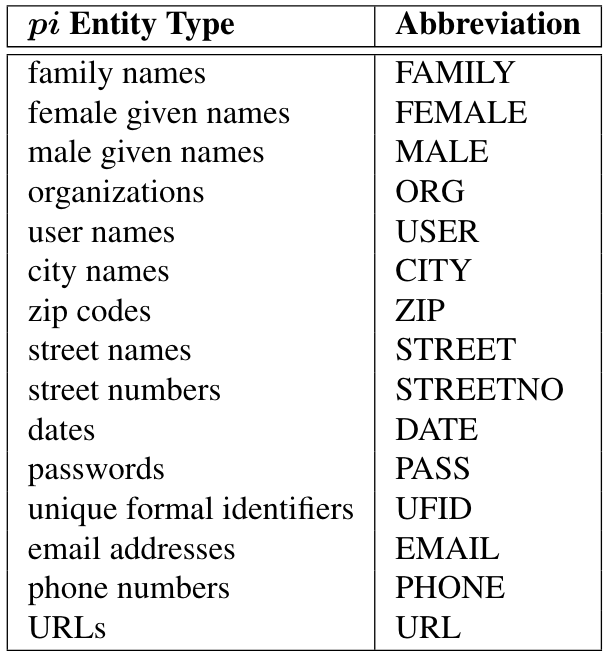
\includegraphics[width=0.55\linewidth]{img/eder-et-al-2.png}
\end{figure}

\begin{tikzpicture}[overlay, remember picture]
\node at (current page.north east)[ref] {
\fullcite{Eder.et.al.2022.LREC} \par};
\end{tikzpicture}

\end{frame}

\begin{frame}{Case-study: Geman e-mails --- Overview}

\begin{figure}
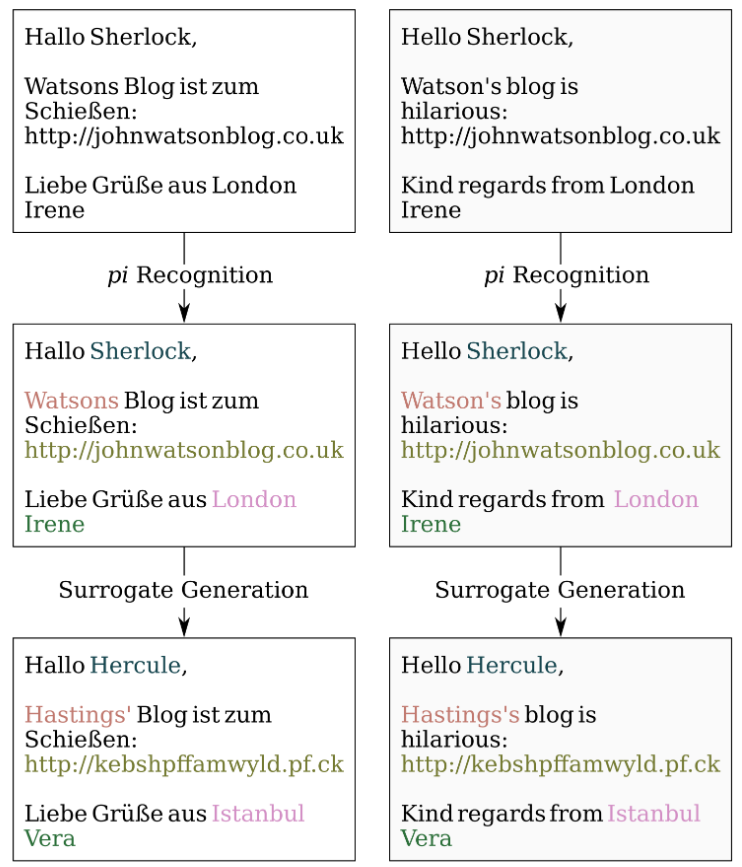
\includegraphics[width=0.50\linewidth]{img/eder-et-al-1.png}
\end{figure}

\begin{tikzpicture}[overlay, remember picture]
\node at (current page.north east)[ref] {
\fullcite{Eder.et.al.2022.LREC} \par};
\end{tikzpicture}

\end{frame}


\begin{frame}{Case-study: Geman e-mails --- Evaluation}

BIO scheme: `B' --- Beginning of an entity, `I' (Inside) for its continuation, and ‘O’ (Outside) for tokens that do not belong to any pi entity)

Weighted average of precision, recall and F1 score

\begin{figure}
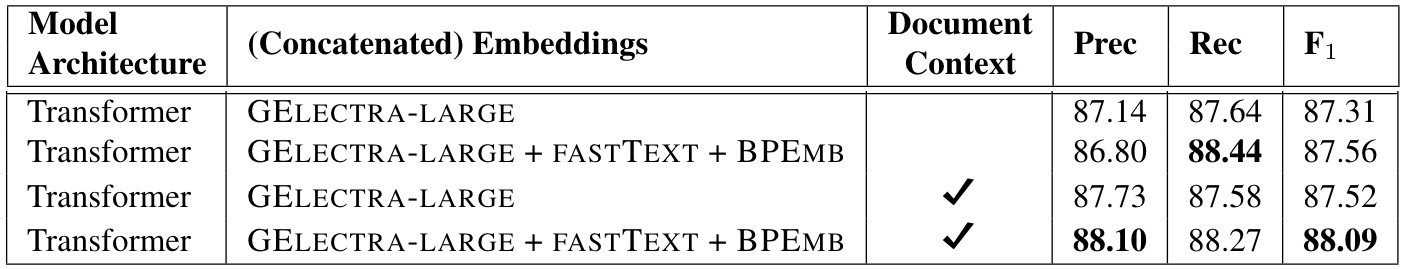
\includegraphics[width=\linewidth]{img/eder-et-al-3}
\end{figure}

How robustly does the system protect privacy?

\begin{tikzpicture}[overlay, remember picture]
\node at (current page.north east)[ref] {
\fullcite{Eder.et.al.2022.LREC} \par};
\end{tikzpicture}

\end{frame}



\begin{frame}{Case-study: MAPA project}

\begin{itemize}
\item 3-level hierarchy of entities: level 1: person, time, location, organization, amount, vehicle
\end{itemize}

\begin{figure}
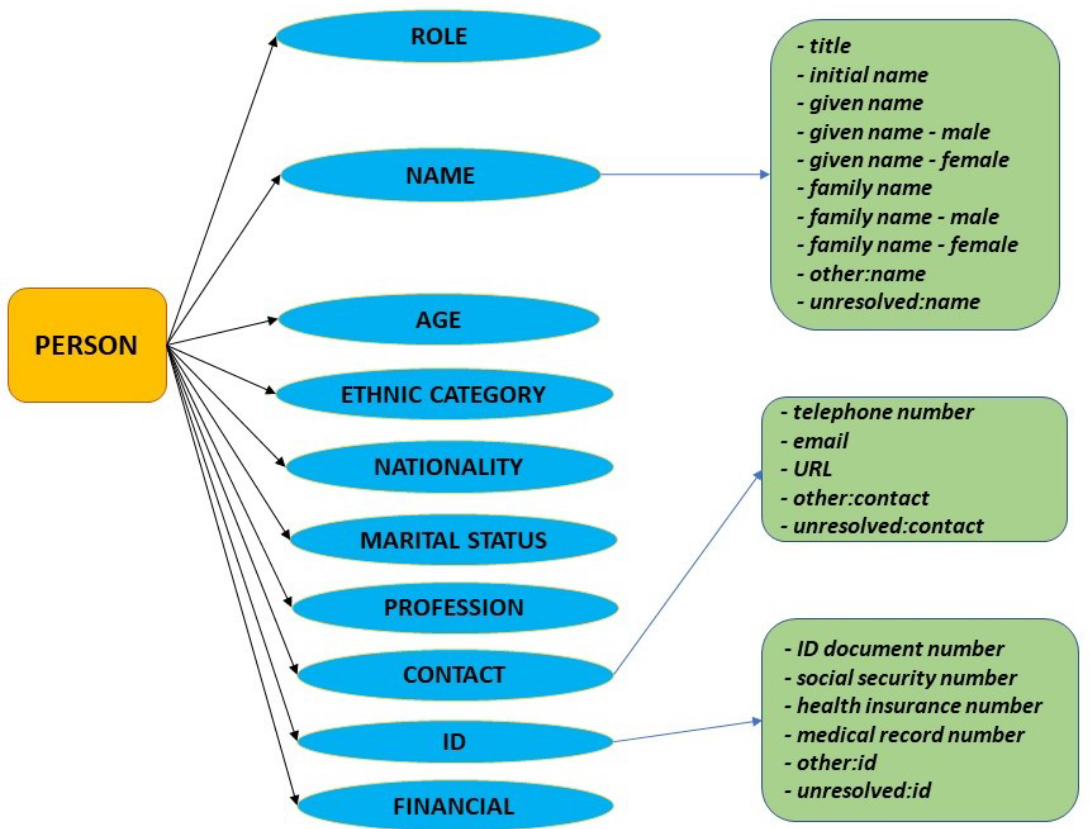
\includegraphics[width=0.48\linewidth]{img/mapa1}
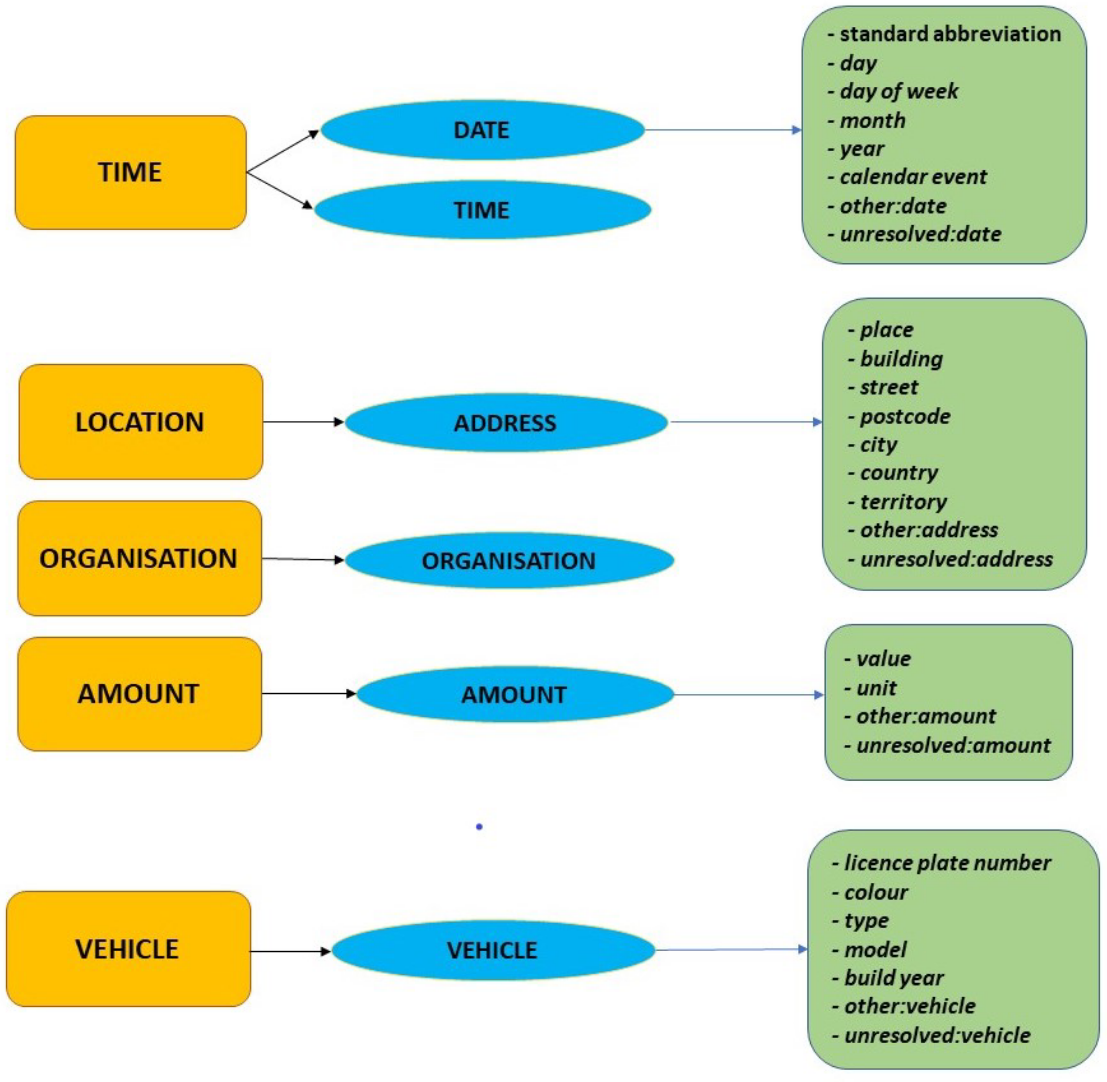
\includegraphics[width=0.48\linewidth]{img/mapa2}
\end{figure}


\begin{tikzpicture}[overlay, remember picture]
\node at (current page.north east)[ref] {
\fullcite{Arranz.et.al.2022.WS} \par};
\end{tikzpicture}

\end{frame}





\begin{frame}{Case-study: MAPA project}

\begin{itemize}
\item  NER model: BERT
\item  Classification only in 2 levels of hierarchy
\item  Rntity replacement: random or using a LM
\item  Datasets: EUR-LEX (2k sentences per lang)
\item  Medical data: created “fake ones” in French by replacing “he”, “she”, “the patient” with fake names
\item  Also some legal judgment in Spanish
\item  Annotated data machine-translated
\end{itemize}

\begin{tikzpicture}[overlay, remember picture]
\node at (current page.north east)[ref] {
\fullcite{Arranz.et.al.2022.WS} \par};
\end{tikzpicture}
\end{frame}




\begin{frame}{Case study: Pseudonymization with LLMs}

\begin{itemize}
\item Pseudonymization adopted from \citet{Eder.et.al.2022.LREC} --- recognize and replace entities
\item Tested 3 approaches: NER, seq2seq (enc-dec), LLM with zero shot
\item 3 classes of entities: PER, LOC, ORG
\item Spacy for NER; for LLM they use GPT-3 and ChatGPT
\item Downstream test on pseudoanonym. data -> summarization (CNN daily mail, standard) and classification (IMDB, standard)
\item Results: on summarization drop in BLEU (quite a big one), on sentiment very little (why?)
\end{itemize}


\begin{tikzpicture}[overlay, remember picture]
\node at (current page.north east)[ref] {
\fullcite{Yermilov.et.al.2023.TrustWS} \par};
\end{tikzpicture}
\end{frame}


\begin{frame}{Case study: TAB Project}

1,268 En cases from ECHR (Introduction and Facts sections)

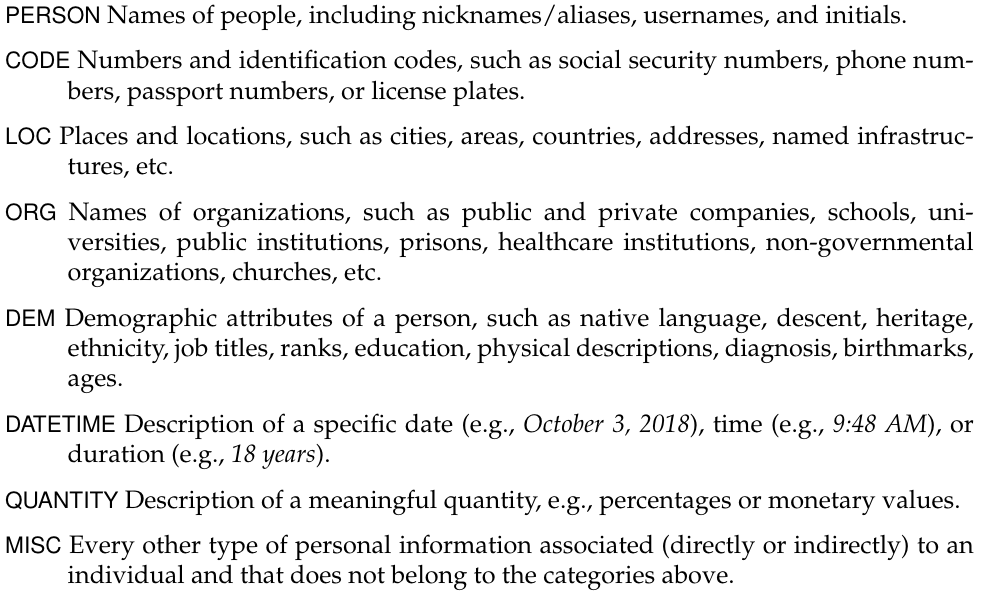
\includegraphics[width=0.9\linewidth]{img/tab1}

\begin{tikzpicture}[overlay, remember picture]
\node at (current page.north east)[ref] {
\fullcite{Pilan.et.al.2022.coli} \par};
\end{tikzpicture}
\end{frame}


\begin{frame}{Case study: TAB Project}

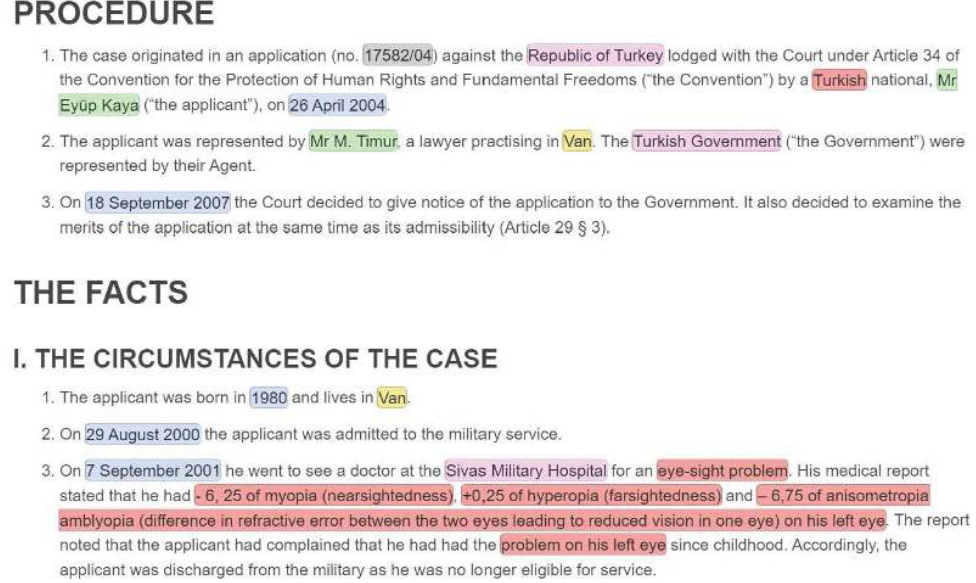
\includegraphics[width=\linewidth]{img/tab2}

\begin{tikzpicture}[overlay, remember picture]
\node at (current page.north east)[ref] {
\fullcite{Pilan.et.al.2022.coli} \par};
\end{tikzpicture}
\end{frame}


\begin{frame}{Case study: TAB Project --- Evaluation}

Evaluation - recall of PII = privacy protection, precision of PII = utility

Absolute recall --- relies on a uniform weight over all annotated identifiers and thus fails to account for the fact that some (quasi-)identifiers have a much larger influence on the disclosure risk than others

Evaluation of anonymization methods is the need to compute the recall at the level of entities rather than mentions. Whenever an entity is mentioned several times in a given document, it only makes sense to view this entity as “protected” if all of its mentions are masked.

\begin{tikzpicture}[overlay, remember picture]
\node at (current page.north east)[ref] {
\fullcite{Pilan.et.al.2022.coli} \par};
\end{tikzpicture}
\end{frame}


\begin{frame}{Case study: TAB Project --- New metrics}

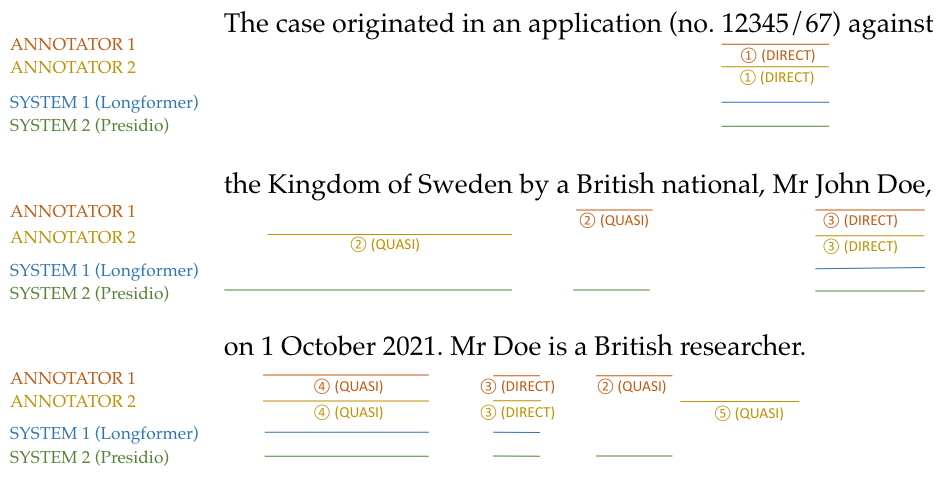
\includegraphics[width=0.7\linewidth]{img/tab3}

Entity is correctly masked if and only if the anonymization model manages to completely mask all of its mentions

Separate recall measures for the direct id (person’s names, case numbers, etc.) and the quasi-id (dates, locations, etc.)

\begin{tikzpicture}[overlay, remember picture]
\node at (current page.north east)[ref] {
\fullcite{Pilan.et.al.2022.coli} \par};
\end{tikzpicture}
\end{frame}

\section{Discussion}

\begin{frame}{Presidio}

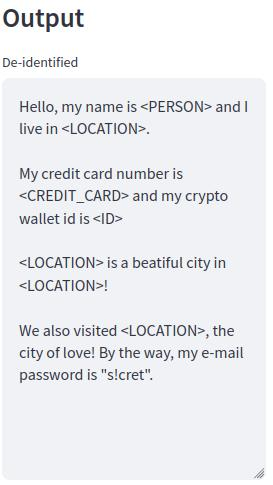
\includegraphics[width=0.35\linewidth]{img/presidio-out}
\pause
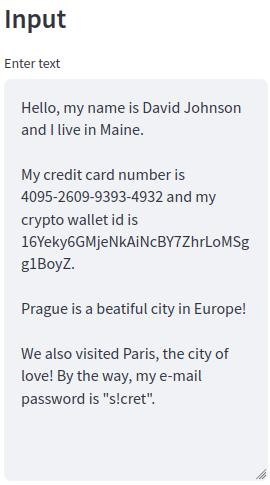
\includegraphics[width=0.35\linewidth]{img/presidio-in}

\end{frame}



\begin{frame}{Limits of anonymization?}
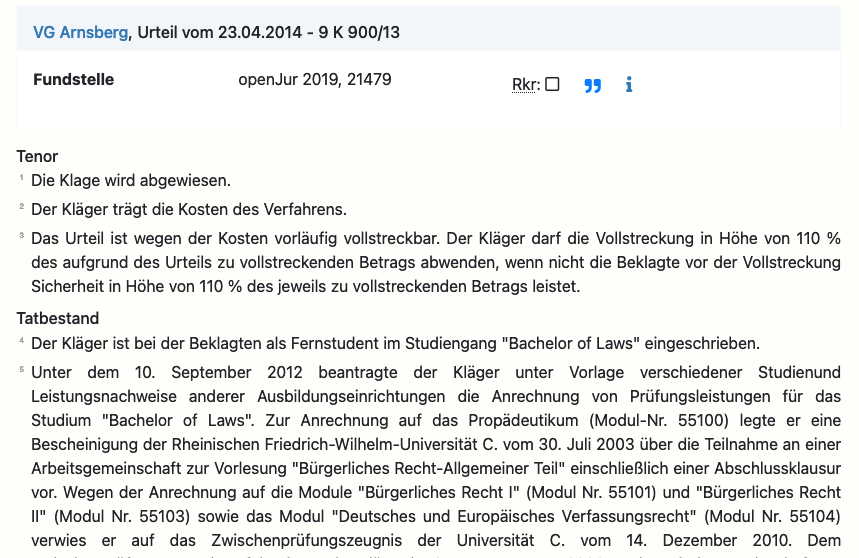
\includegraphics[width=0.95\linewidth]{img/hagen2}
\end{frame}




\begin{frame}{Exercise}
Build your own text anonymizer
\begin{itemize}
\item Get existing dataset (see the case studies)
\item Fine-tune a small BERT transformer model (or RNN tagger)
\item Evaluate quantitatively and explore errors manually
\end{itemize}
\end{frame}



\begin{frame}{License and credits}

	\begin{columns}
		\begin{column}{0.7\textwidth}
			Licensed under Creative Commons Attribution-ShareAlike 4.0 International (CC BY-SA 4.0)
		\end{column}
		\begin{column}{0.2\textwidth}
			
\includegraphics[width=0.9\linewidth]{img/cc-by-sa-icon.pdf}
		\end{column}
	\end{columns}
	
	\bigskip
	
	Credits
	
	\begin{scriptsize}
		
		Ivan Habernal
		
		Content from ACL Anthology papers licensed under CC-BY \url{https://www.aclweb.org/anthology}
		
		Partly inspired by lectures from Antti Honkela, Aurélien Bellet, Gautam Kamath
	
	\end{scriptsize}
	
\end{frame}




\end{document}

